\chapter{Konzept}

\label{AppendixKonzept}

\section{Design- und Bedienkonzept}\label{design--und-bedienkonzept}

\subsection{Mockups}

\subsubsection{Homepage}

\begin{figure}[!htb]
  \centering
  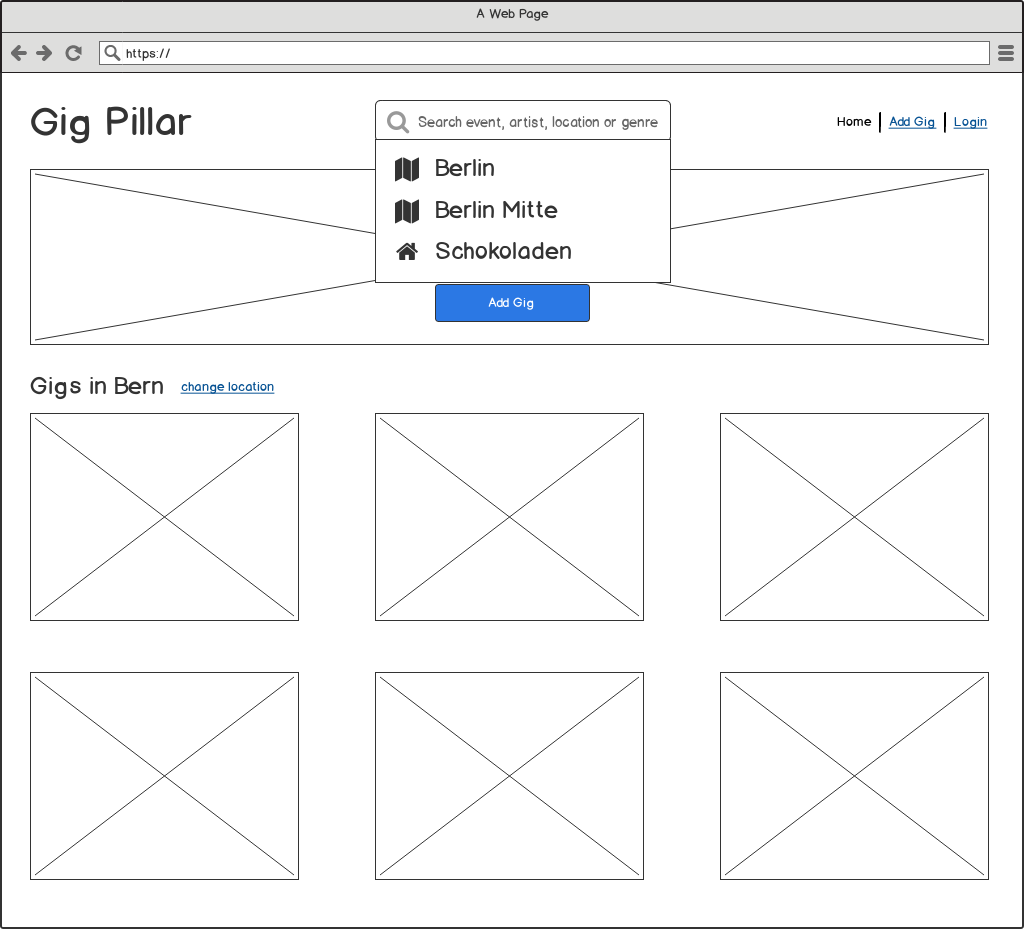
\includegraphics[width=0.95\textwidth]{mockups/homepage.png}
  \caption{Mockup: Homepage}
\end{figure}

\clearpage
\subsubsection{Suchresultate}

\begin{figure}[!htb]
  \centering
  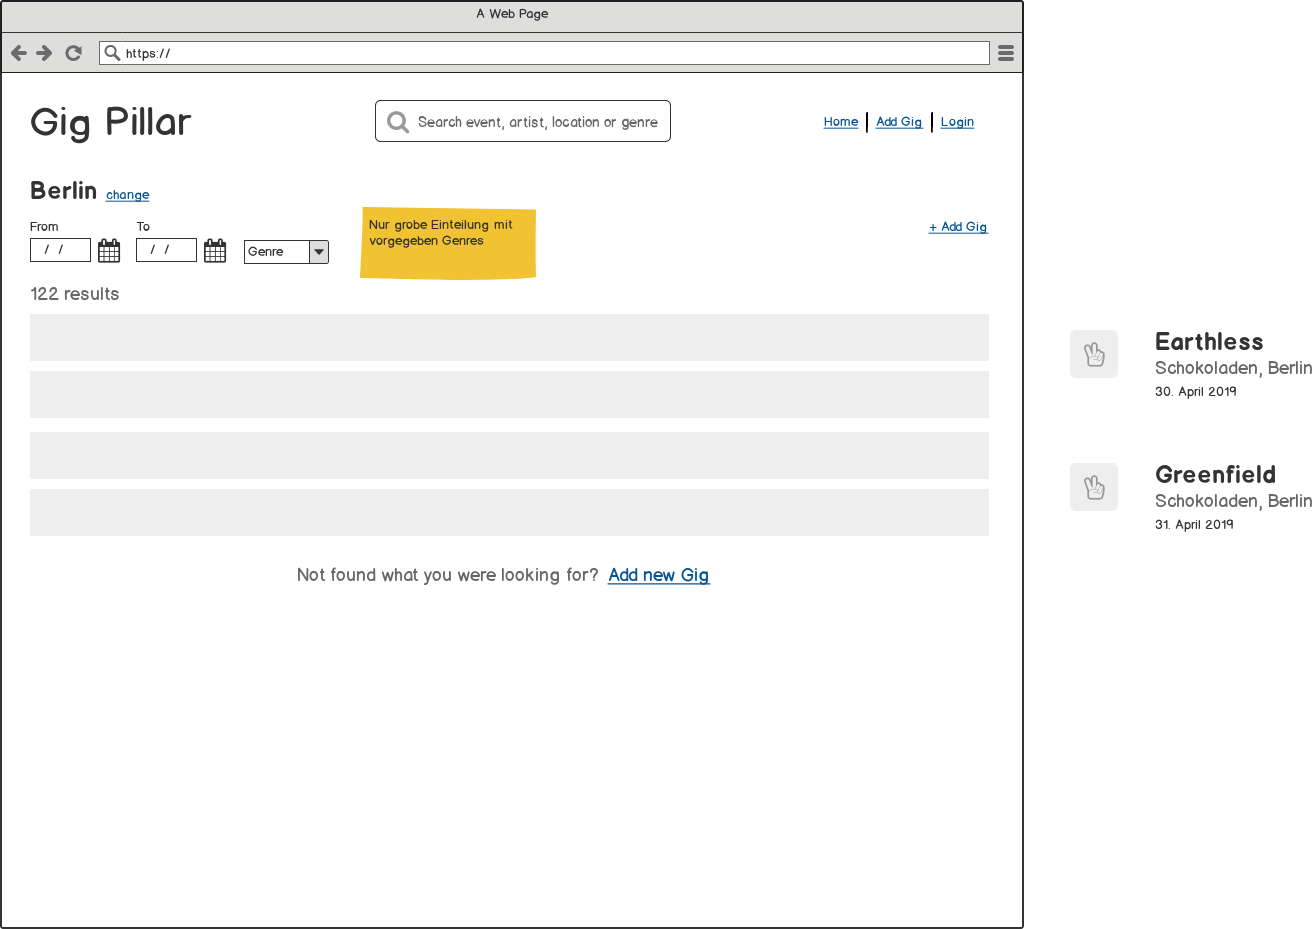
\includegraphics[width=0.95\textwidth]{mockups/search-result.png}
  \caption{Mockup: Suchresultate}
\end{figure}

\clearpage
\subsubsection{Gig Ansicht}

\begin{figure}[!htb]
  \centering
  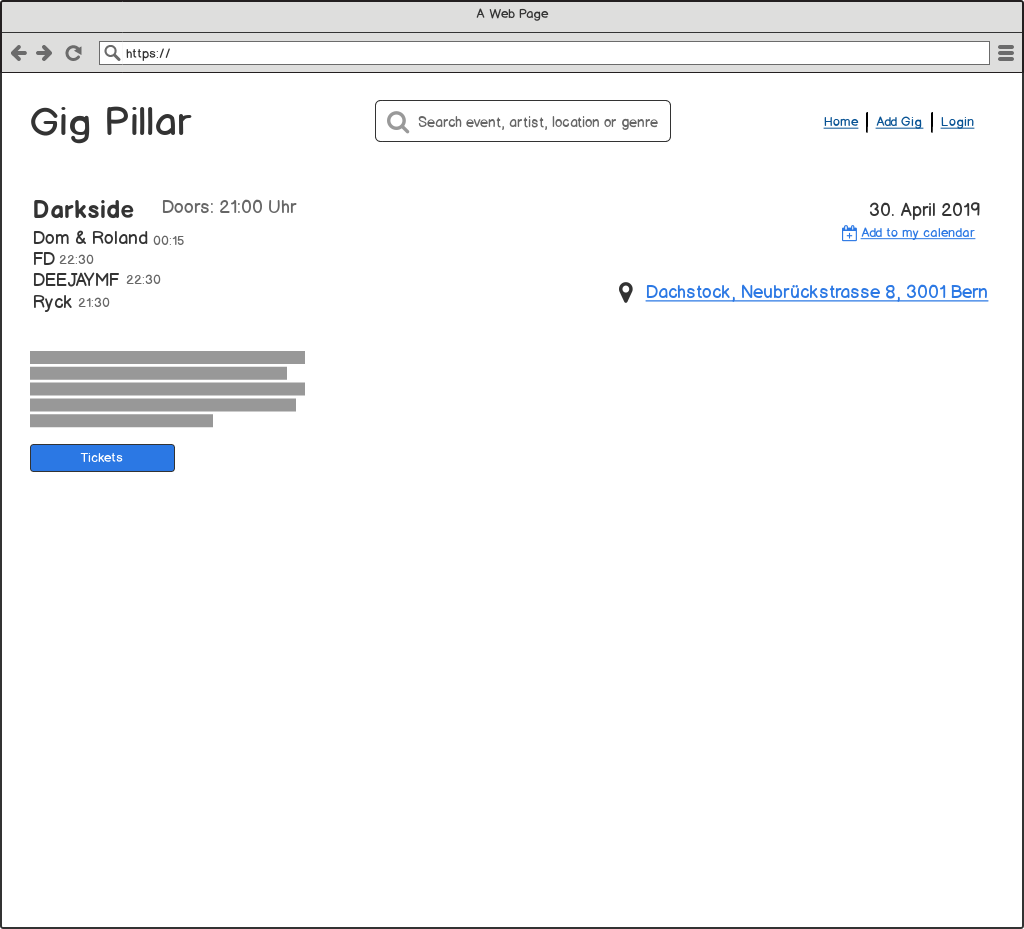
\includegraphics[width=0.95\textwidth]{mockups/event.png}
  \caption{Mockup: Gig Ansicht}
\end{figure}

\clearpage
\subsubsection{Gig erfassen}

\begin{figure}[!htb]
  \centering
  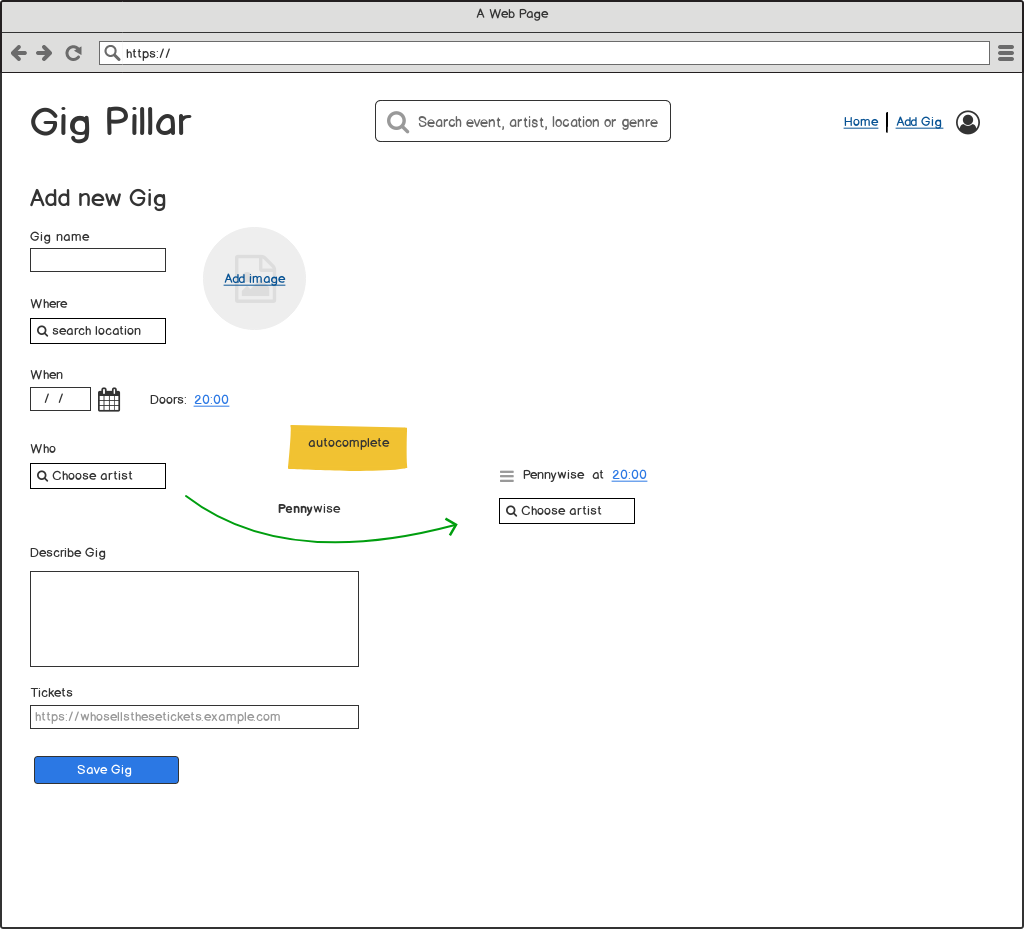
\includegraphics[width=0.95\textwidth]{mockups/add-gig.png}
  \caption{Mockup: Gig erfassen}
\end{figure}

\clearpage
\subsubsection{Benutzerprofil}

\begin{figure}[!htb]
  \centering
  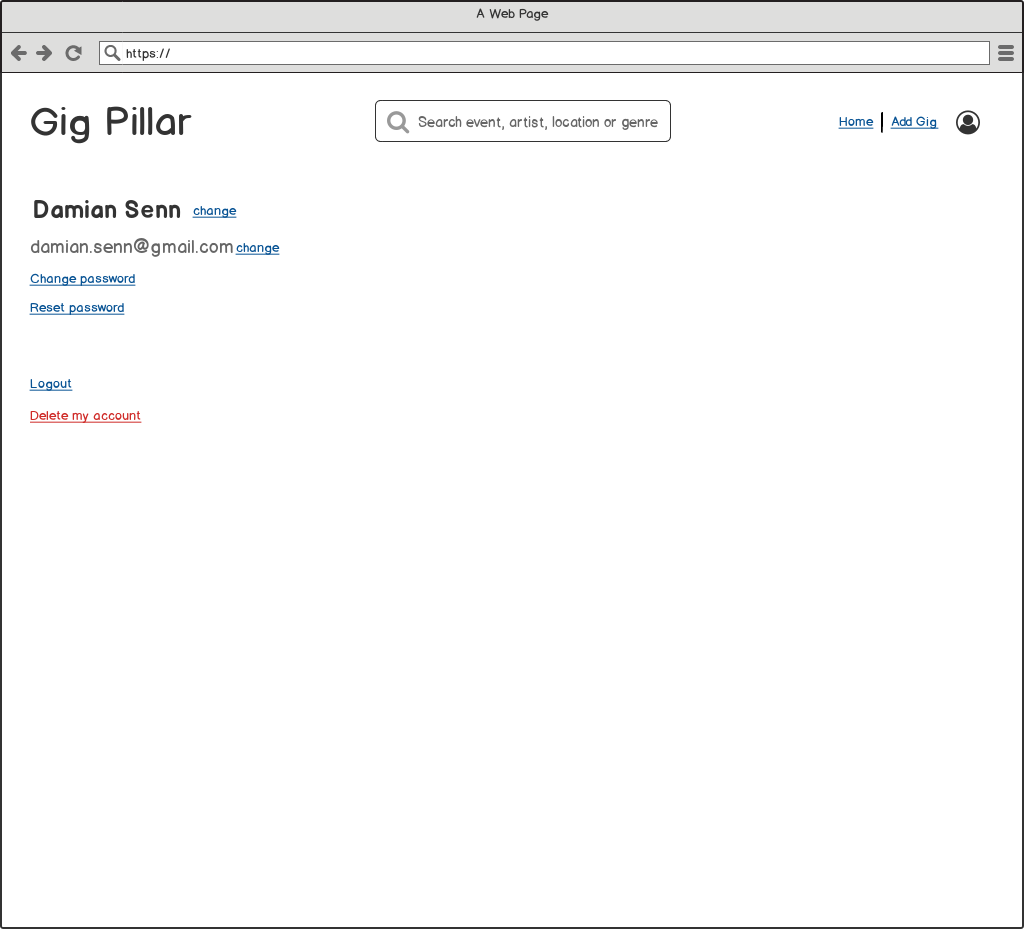
\includegraphics[width=0.95\textwidth]{mockups/profile.png}
  \caption{Mockup: Benutzerprofil}
\end{figure}

\clearpage
\section{Softwarekonzept}\label{softwarekonzept}

\section{Testkonzept}\label{testkonzept}
